\section{Concrete implementation}
\label{sec:concrete}

\Red{In this section I only talk about TSNI.  Once we finish the previous
  section to both talk about TSNI and TINI, we should do the same here.}

The operational semantics we have derived in the previous section
satisfy termination sensitive non-interference by design.  However,
these abstract semantics essentially require that different tasks
execute completely isolated.  For instance, for the mini-ML language,
this means that every task has it's own heap.  For practical
implementations this is often not desirable.  Instead, we would like to
more tightly couple the integration of the target and IFC
language by reusing existing infrastructure.  In the running example,
a concrete implementation might use a single global heap, and ensure
that references do not cross task boundaries, and thus preserving
non-interference.

In this section, we will detail an approach that allows one to implement
a concrete system differently from our proposal in the previous
section, and give conditions for when such a system preserves termination
sensitive non-interference.
We explain the idea for the single heap mini-ML language, and then
generalize to arbitrary systems.

\subsection{IFC-Mini-ML with a Single Heap}

Instead of using a configuration of the form
|iconf iS (fullconf id1 il1 tS1 ie1, fullconf id2 il2 tS2 ie2 ldots)|
where every task has its
own ML heap, we would like a single global heap as in
|oneheapiconf iS tS (oneheapfullconf id1 il1 ie1, oneheapfullconf id2 il2 ie2, ldots)|.
Furthermore, we keep up a fictional separation between the portions
of the global heap that tasks can use by forbidding references to
cross task boundaries. Most
of the operational rules can easily be adapted to work with these
new configurations.  In the abstract system, the \textsc{I-fork}
rule created a new heap for the new task to execute in.  Since we
want to forbid references to cross task boundaries, we do not modify
the global heap and instead add an additional premise that the forked
expression |ie| must not contain any references.
Finally, we add the same condition to the \textsc{I-send} rule.
Tasks that try to fork or send an expression that contains a
reference will now get stuck, and will stop executing by the
\textsc{I-noStep} rule.

\Red{Show the key rules here.}

As we have outlined the IFC-Mini-ML language with a single heap, we
effectively restrict the abstract semantics in some cases (namely
to not allow the passing of references) as well as using a different
way to represent the heap.  How can we be sure that these
new, \textit{concrete semantics} for our system still satisfy
termination-sensitive non-interference?

Intuitively, there are two scenarios in which non-interference
can be violated when restricting the transition relation:
\begin{itemize}
  \item Adding an additional premise to one of the rules that inspects
  information which is above the security label of the task currently
  executing.  This would allow another task to observe the termination
  of the other if both are at the same security level, and thus observe
  the secret information that was used in the additional
  premise of the rule.
  \item Adding additional restrictions to transition rules can
  also cause the whole configuration to get stuck, which can leak
  information through the termination channel.
\end{itemize}

%This isn't trivial, as it is not sound to add arbitrary additional
%conditions on evaluation rules.  To see this, consider a contrived
%concrete system where we add a premise to a reduction rule that
%stops a task based on secret information.  Such a system will
%not satisfy non-interference, as it allows other tasks on the
%same level to observe the termination of that task and thus the
%secret information which was used to decide if the task terminates
%or not.

\subsection{Correctness of Concrete Semantics}

To formalize the conditions under which we can show the concrete
semantics preserve non-interference, we require some notation:

\Red{isomorphism definition here}

Now, we propose the following two-step process to ensure that
TSNI is preserved:
\begin{enumerate}
  \item First, any of the reduction rules of the abstract
  semantics presented in Section~\ref{sec:retrofit} can
  be restricted by adding a predicate $P$ to the premise of
  any rule other than \textsc{I-noStep}.  The predicate $P$
  can depend only on the \textit{erased} configuration
  |erase il ic|, where |il| is the label of the first task
  in the task list.
\end{enumerate}


We now have a concrete semantics, which both uses a different
representation for some of the constructs in language (a single
heap rather than a heap per task in our running example), as well
as restricting some of the operational rules to disallow
undesirable transitions.  To show that the concrete semantics
still satisfy TSNI, we use two techniques.  First, we give a
condition on what kind of restrictions can be allowed on the
operational rules.  Secondly, we define the notation of an
isomorphism between IFC languages and show that it preserves
non-interference.

\Red{At some point in this section we should say a little about
  why the abstract setting needs complete isolation (because it
  works for \textit{any} language), and that this is sometimes
  what you want.}

\subsection{\Red{Previous Stuff (to be merged/removed as necessary)}}

The operational semantics we have derived in the previous section
constitutes an abstract \emph{specification}: a semantics for which
non-interference is (obviously) true.  This specification can guide the
design of an information-flow calculus which would not be directly
derivable from our procedure, but is related to some such derivation.
For example, in our mini-ML language, the combined semantics requires
each thread to have a separate ML heap.  In an actual implementation, we
might like to only have a single heap and disallow the passing of
references between threads.  This restriction maintains a correspondence
between the abstract multiple heaps and the concrete single heap.  We might
hope that we can prove noninterference for this new system by reusing
noninterference for the old system.

However, modifying operational rules poses a distinct problem for
preserving non-interference.  Consider a trivial state machine as shown
in Figure~\ref{fig:trivial-sm}, whose second projection is classified
secret.  With all three transitions, this language fulfills
termination-sensitive noninterference.  Furthermore, if the dashed line
is removed, the language continues to satisfy TSNI.  However, if any
solid line is removed, however, the language fails TSNI.

\begin{figure}
    States: $(x,y)$ for $x,y \in \{0,1\}$ \\
    Erasure function: $f(x,y) = (x,\bullet)$

    \begin{center}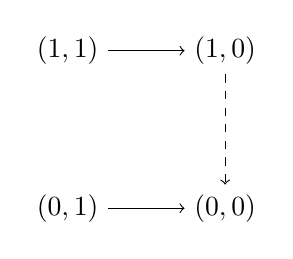
\begin{tikzpicture}[node distance=2cm, auto]
        \node (A) {$(1,1)$};
        \node (B) [right of=A] {$(1,0)$};
        \node (C) [below of=A] {$(0,1)$};
        \node (D) [right of=C] {$(0,0)$};
        \draw[->] (A) to node {} (B);
        \draw[->] (C) to node {} (D);
        \draw[->, dashed] (B) to node {} (D);
    \end{tikzpicture}\end{center}

    \label{fig:trivial-sm}
    \caption{A trivial state machine}
\end{figure}

The approach we will take is in two steps.  First, we sidestep the
restriction problem by demanding that the concrete implementation be
\emph{isomorphic} to the abstract specification, but perhaps having a different
runtime representation (a single heap) and some well-formedness
condition (every item on the heap only contains pointers from a single
location).  Isomorphism will preserve nonintereference, but it will also means all
transitions in the abstract language have to be implemented, including
undesirable transitions such as sending a pointer to another thread makes
the pointer dangling.  Next, we define a desugaring into this language
which adds dynamic checks, eliminating the possibility for these undesirable
transitions to be exercised.

\Red{Move these definitions earlier}

%{
%format tyerase c = "\varepsilon("c")"
%format tyerasef = "\varepsilon"
%format ^ = " "
%format c = "c"
%format c'
%format cc = "\con{"c"}"
%format cc'
%format ac = "\abs{"c"}"
%format ac'
%format finv = f"^{-1}"
%format V = "V"
%format cV = "\con{"V"}"
%format aV = "\abs{"V"}"
%format ~= = "\approx_l"
%format clequiv = "\con{"~="}"
%format alequiv = "\abs{"~="}"
%format creduce = "\con{".->"}"
%format areduce = "\abs{".->"}"
%format creducestar = "\con{".=>"}"
%format areducestar = "\abs{".=>"}"
%format (ap (f) (x)) = f"("x")"
%format .. = "\circ"
%format idf (t) = "id_{"t"}"

\begin{definition}[Information-flow control language]
    An information-flow control language L is a tuple |(C, .->,
    erasef l)|, where $c \in |C|$ is the type of machine configurations, |.->| is a
    reduction relation between machine configurations and |erasef l : C .-> tyerase C|
    is an erasure function parametrized on labels from machine configurations to \emph{erased} machine
    configurations |tyerase C|.  For sequential languages, the
    language is augmented with a set of terminal configuration states $V
    \subseteq |C|$ for which there are no possible further transitions.
\end{definition}

\begin{definition}[$l$-equivalence]
    In a language |(C, .->, erasef l)|, two machine configurations
    |memberf (c, c') C| are considered $l$-equivalent (|c ~= c'|)
    if |erase l c = erase l c'|.
\end{definition}

\newcommand{\con}[1]{\ensuremath{{\color{red} #1}}}
\newcommand{\abs}[1]{\ensuremath{{\color{blue} #1}}}

Before we show isomorphism preserves termination sensitive
non-interference, we'd like to remark that one can safely remove transitions
and preserve termination \emph{insensitive} interference:

\begin{definition}[Weak isomorphism of information-flow control languages]
    A language \con{|(C, .->, erasef l)|} is weakly isomorphic to a
    language \abs{|(iC, .->, erasef l)|} if there exist total functions
    |f : tC -> iC| and |finv : iC -> tC| such that |f .. finv = idf tC|
    |finv .. f = idf iC|.  Furthermore, the following coherence conditions
    must hold:
    \begin{itemize}
        \item |f| is functorial (e.g. if $\abs{x\ R\ y}$ then
            $f(\abs{x})\ \con{R}\ f(\abs{y})$) over both
            $l$-equivalences and |.->|, and
        \item |finv| is functorial over $l$-equivalence (though not necessarily |.->|).
    \end{itemize}
\end{definition}

\begin{theorem}[Weak isomorphism preserves termination insensitive non-interference]
    If a language \con{L} is included in a language \abs{L}, and \abs{L}
    satisfies TINI, then \con{L} satisfies TINI.
\end{theorem}

\begin{proof}
    Shown by transporting configurations and reduction derivations
    from \con{L} to \abs{L}, applying TINI and transporting the resulting
    equivalence back using functoriality of |finv| over $l$-equivalences.
\end{proof}

Isomorphism requires that |finv| is functorial over reduction relations
as well, i.e. that we can extract a concrete reduction sequence from an abstract one.

\begin{definition}[Isomorphism of information-flow control languages]
    A language \con{|(C, .->, erasef l)|} is
    isomorphic to a language \abs{|(iC, .->, erasef l)|} if there exist total functions
    |f : tC -> iC| and |finv : iC -> tC| such that |f .. finv = idf tC|, |finv .. f = idf iC|, and both |f| and |finv| are
    functorial over both $l$-equivalences and |.->|.
%(if |cc clequiv
%   cc'| then
%   |(ap f cc) alequiv (ap f cc')| and if |ac alequiv ac'|
%   then |(ap finv ac) clequiv (ap finv ac')|) and
%   |.->| (if
%   |cc creduce cc'| then |(ap f cc) areduce (ap f cc')| and
%   if |ac areduce ac'| then |(ap finv ac) creduce (ap finv ac')|)
\end{definition}

\begin{theorem}[Isomorphism preserves termination sensitive non-interference]
    If \ifc{L} is isomorphic to \tar{L} and \ifc{L} satisfies TSNI, then
    \tar{L} satisfies TSNI.
\end{theorem}

\begin{proof}
    Shown by transporting configurations and reduction derivations from
    \tar{L} to \ifc{L}, applying TSNI, and then transporting the
    resulting configuration, $l$-equivalence and multi-step derivation back.
\end{proof}
%}



\begin{figure}

\begin{mathpar}
\inferrule[I-stepT]
{|
conf tS (te) -> conf tS' te'
|}
{|
coconf iS tS (cconf id il (iniE (IT te)), ldots)
.->
iS ; tS' ; sched step (cconf id il (iniE (IT te')), ldots)
|}

\and
% This rule is not complete, needs the FV condition
\inferrule[C-fork]
{ 
|iS' = iS [ id' mapsto nil ]|\\
|it1 = cconf id il (iniE id')|\\
|itnew = cconf id' il (TI ie)|\\
|fresh (id')|
}
{|
coconf iS tS (lconf id il (iniE (fork ie)), ldots)
.->
iS'; tS; sched fork (it1, ldots, itnew)
|}
\end{mathpar}

\caption{ML with a single heap}
\label{fig:comb}
\end{figure}

This version
